\subsection{Innovative task: Minimum Spanning Tree}
\subsubsection{Proof of Correctness}
In order to verify the correctness of our implementation, we first run our algorithm on tiny synthetic graph with 10 nodes and 17 edges. We verified the result is correct. Then we compare our implementation against MATLAB's implementation of Minimum Spanning Tree and we get identical result for output of both implementation.

\subsubsection{Experiment on Large datasets}
Since MST algorithm require that graph is fully connected, weighted, and undirected. We can barely find such graph in Konect and SNAP project. Therefore, we generate synthetic graph of different size. We plot the runtime against graph size (number of nodes) in Figure \ref{mst:fig}. We find the run time grows near-quadratically as the number of nodes in graph. This is identical to the time complexity of Prim's Algorithm, which is $O(N^2)$.

\begin{figure}[!htbf]
\begin{center}
     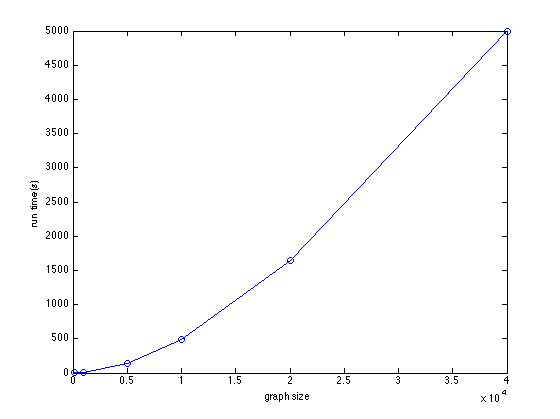
\includegraphics[width=0.8\textwidth]{FIG/mst.png} 
\caption{MST runtime plot}
\label{mst:fig}
\end{center}
\end{figure}
